%%!TEX root = main.Rnw
%\documentclass[class=article, crop=false]{standalone}
%\ifstandalone
%\usepackage{haziq_article}
%\fi
%\begin{document}



We can include some R code here. Hello

\begin{knitrout}
\definecolor{shadecolor}{rgb}{1, 1, 1}\color{fgcolor}\begin{kframe}
\begin{alltt}
\hlkwd{library}\hlstd{(iprior)}
\hlstd{mod} \hlkwb{<-} \hlkwd{ipriorOptim}\hlstd{(}\hlkwd{kernL}\hlstd{(y} \hlopt{~} \hlstd{.} \hlopt{^} \hlnum{2}\hlstd{,} \hlkwc{data} \hlstd{= simdat))}
\end{alltt}
\begin{verbatim}
## Iteration 0:    Log-likelihood = -491.76134 
## Iteration 1:    Log-likelihood = -452.90519 ........
## Iteration 2:    Log-likelihood = -417.44265 .......
## Iteration 3:    Log-likelihood = -393.65504 .......
## EM NOT CONVERGED!
## 
## Now switching to optim...
## 
## iter   10 value 259.621574
## iter   20 value 255.501753
## final  value 255.454420 
## converged
## 
## Preparing iprior output... DONE.
\end{verbatim}
\begin{alltt}
\hlkwd{print}\hlstd{(mod)}
\end{alltt}
\begin{verbatim}
## 
## Call:
## iprior(formula = y ~ .^2, data = simdat)
## 
## RKHS used: Pearson & Canonical, with multiple scale parameters.
## 
## 
## Parameter estimates:
## (Intercept)     lambda1     lambda2         psi 
##  1.74493392  0.46809945  0.02367604  3.61187777
\end{verbatim}
\end{kframe}
\end{knitrout}
\begin{knitrout}
\definecolor{shadecolor}{rgb}{1, 1, 1}\color{fgcolor}\begin{figure}[h]

{\centering 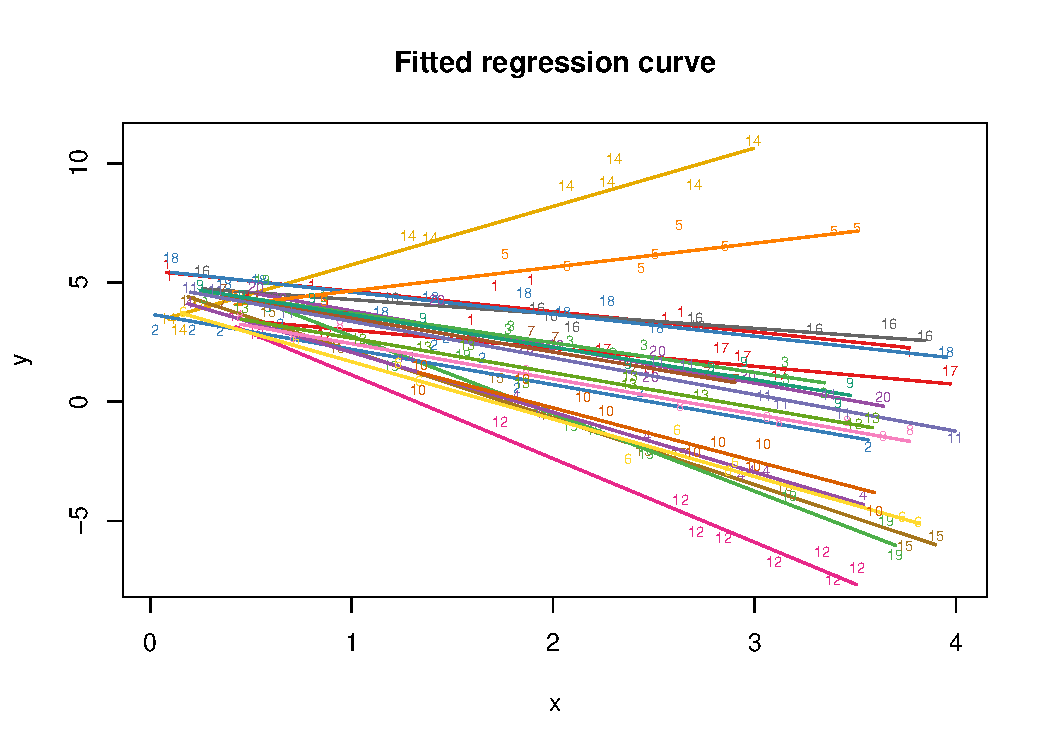
\includegraphics[width=\maxwidth]{figure/iprior_plot-1} 

}

\caption[This is a caption]{This is a caption.}\label{fig:iprior.plot}
\end{figure}


\end{knitrout}

The plot in Figure \ref{fig:iprior.plot} is explained in further detail in \cite{jamil2017}. Notice that I have used a reference to the figure via \verb@\ref{fig:<name-of-chunk>}@. The following shows a side-by-side plot. We can also reference them Figure \ref{fig:iprior.residplot1} and Figure \ref{fig:iprior.residplot2}.

\begin{knitrout}
\definecolor{shadecolor}{rgb}{1, 1, 1}\color{fgcolor}\begin{figure}
\subfloat[The left plot.\label{fig:iprior.residplot1}]{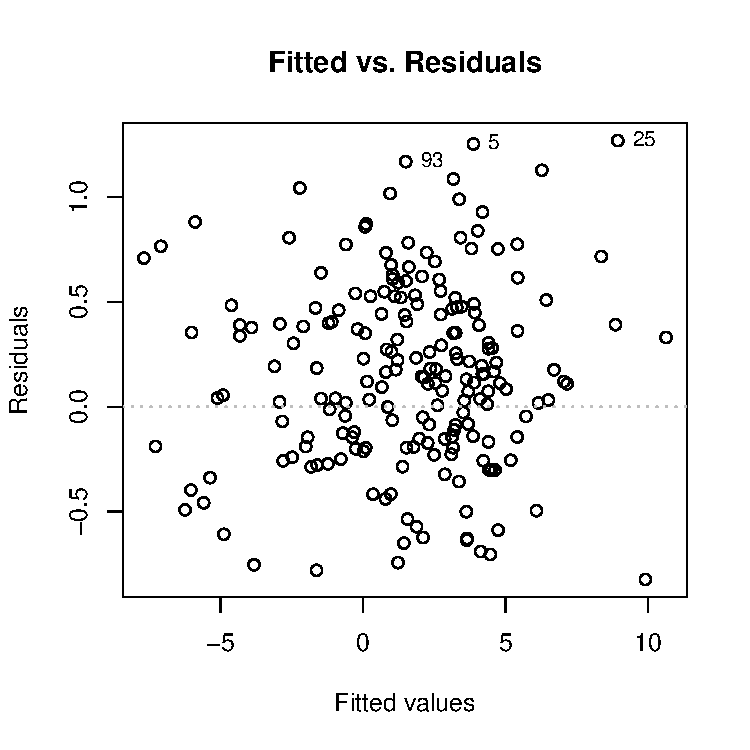
\includegraphics[width=7cm,height=7cm]{figure/iprior_residplot-1} }
\subfloat[And the right one.\label{fig:iprior.residplot2}]{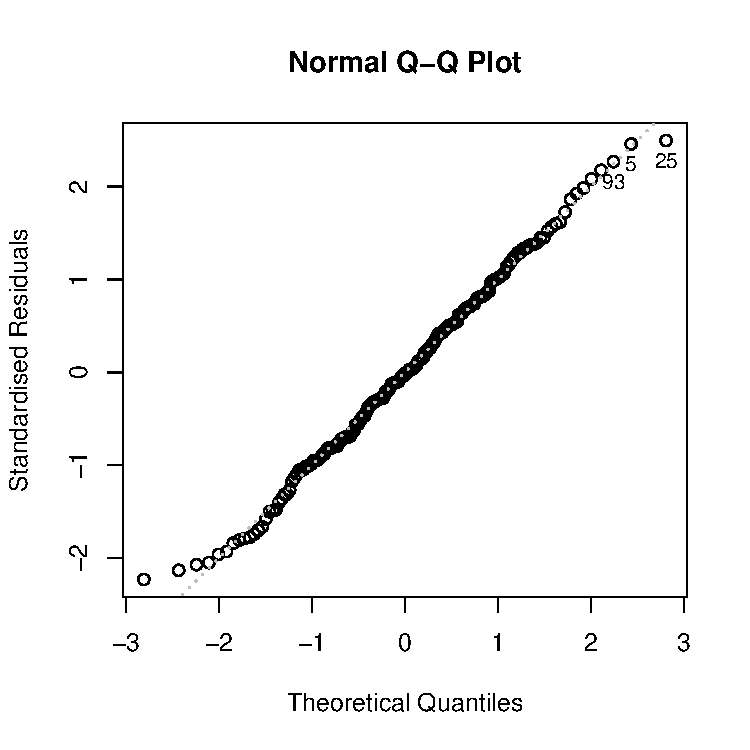
\includegraphics[width=7cm,height=7cm]{figure/iprior_residplot-2} }\caption[Side-by-side plot]{Side-by-side plot}\label{fig:iprior.residplot}
\end{figure}


\end{knitrout}

%%%%%%%%%%%%%%%%%%%%%%%%%%%%%%%%%%%%%%%%%%%%%%%%%%%%%%%%%%%%%%%%%%%%%%%%
%%% REFERENCES %%%%%%%%%%%%%%%%%%%%%%%%%%%%%%%%%%%%%%%%%%%%%%%%%%%%%%%%%
%%%%%%%%%%%%%%%%%%%%%%%%%%%%%%%%%%%%%%%%%%%%%%%%%%%%%%%%%%%%%%%%%%%%%%%%
%\ifstandalone
%\nocite{*}
%\bibliographystyle{apalike}
%\bibliography{haziq}
%\fi

%\end{document}


